% Created 2020-06-01 Mon 18:31
% Intended LaTeX compiler: pdflatex
\documentclass[11pt]{article}
\usepackage[utf8]{inputenc}
\usepackage[T1]{fontenc}
\usepackage{graphicx}
\usepackage{grffile}
\usepackage{longtable}
\usepackage{wrapfig}
\usepackage{rotating}
\usepackage[normalem]{ulem}
\usepackage{amsmath}
\usepackage{textcomp}
\usepackage{amssymb}
\usepackage{capt-of}
\usepackage{hyperref}
\author{Eric Nguyen}
\date{December 12, 2018}
\title{A Look at Atmospheric CO\(_{\text{2}}\)}
\hypersetup{
 pdfauthor={Eric Nguyen},
 pdftitle={A Look at Atmospheric CO\(_{\text{2}}\)},
 pdfkeywords={},
 pdfsubject={},
 pdfcreator={Emacs 26.3 (Org mode 9.1.9)}, 
 pdflang={English}}
\begin{document}

\maketitle
\tableofcontents


\section{Description}
\label{sec:org91827ea}

The original document can be found at
\url{http://sustainabilitymath.org/word/Mauna-Loa-CO2.docx}. \\

\noindent A Look at Atmospheric CO\(_{\text{2}}\) \\
Produced by Thomas J. Pfaff \\
Ithaca College \\
Updated June 2018 \\

\begin{figure}[htbp]
\centering
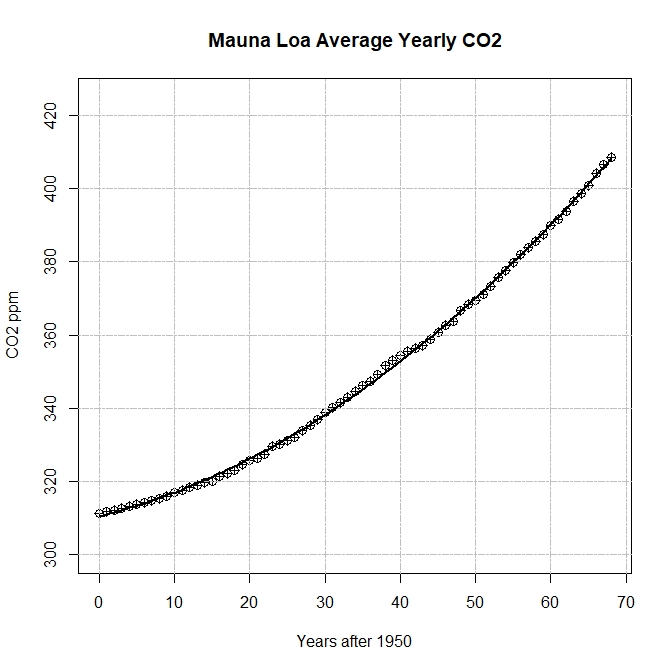
\includegraphics[width=.9\linewidth]{./figures/figure-01.jpg}
\caption{\label{fig:org6bd9d10}
Figure 1 Atmospheric CO2 data, 1950-2017, from the Mauna Loa site, \url{ftp://aftp.cmdl.noaa.gov/products/trends/co2/co2\_annmean\_mlo.txt}, with a fitted curve.}
\end{figure}

\subsection{Note}
\label{sec:org12b3cff}

According to Warren\footnote{According to IPCC Fifth Assessment Report (AR5) page 22: \url{https://www.ipcc.ch/pdf/assessment-report/ar5/syr/AR5\_SYR\_FINAL\_SPM.pdf}}, at \(1^{\circ}\) Celsius, in addition to the trends
we are already observing, oceans will further acidify, natural
ecosystems will start to collapse, and as many as 18-60 million people
in the developing world will go hungry.
At \(1.5^{\circ}\) Celsius the Greenland ice sheet will melt, eventually causing
a 7m rise in sea level, inundating coastal areas.
At \(2^{\circ}\) Celsius agricultural yields in the rich nations will start to
fall and 1-3 billion people will experience water scarcity.
At \(3^{\circ}\) Celsius the Amazon rainforest is expected to collapse and at
\(4^{\circ}\) Celsius most of Africa and Australia will lose all agricultural
production.

\section{Questions}
\label{sec:orgc778e3d}

Answer the following questions using the fitted curve,
\(\hat{y} = 310.42336317 + 0.52063260x + 0.01345947x^2\),
that is represented in \hyperref[fig:org6bd9d10]{Figure 1}.

\subsection{Question 1}
\label{sec:org98ee15e}

Find a model with output Average MH4 in PPB and input years (or years after 1950).
[Either delete this question or the figure, in which case provide the data.]

\noindent\rule{\textwidth}{0.5pt}

First, we need to extract the data from the 'data.txt' file.

\begin{verbatim}
# This code snippet extracts the data from 'data.txt'
%config InlineBackend.figure_format='retina'

import numpy as np
import matplotlib.pyplot as plt
import pandas as pd

data = pd.read_csv("data.txt")

# Years after 1950, instead of actual years
data["year"] = data["year"] - 1950

# Print head
head = data.head()
[list(head)] + [None] + head.values.tolist()
\end{verbatim}

\begin{center}
\begin{tabular}{rrr}
year & mean & unc\\
\hline
9.0 & 315.97 & 0.12\\
10.0 & 316.91 & 0.12\\
11.0 & 317.64 & 0.12\\
12.0 & 318.45 & 0.12\\
13.0 & 318.99 & 0.12\\
\end{tabular}
\end{center}

Once we've extracted the data, we can make a visualization.

\begin{verbatim}
# This code snippet plots the data from 'data.txt'
def plot_config(size=(10, 10),
                xlab = "Years after 1950",
                ylab = "ppm"):
    plt.figure(figsize=size)
    plt.xlabel(xlab)
    plt.ylabel(ylab)
    plt.grid()

def scatterplot():
    plot_config()
    plt.scatter(data["year"],
                data["mean"],
                marker="s",
                facecolors="none",
                edgecolors="black")

scatterplot()
plt.savefig("figures/data.png")
\end{verbatim}

\begin{center}
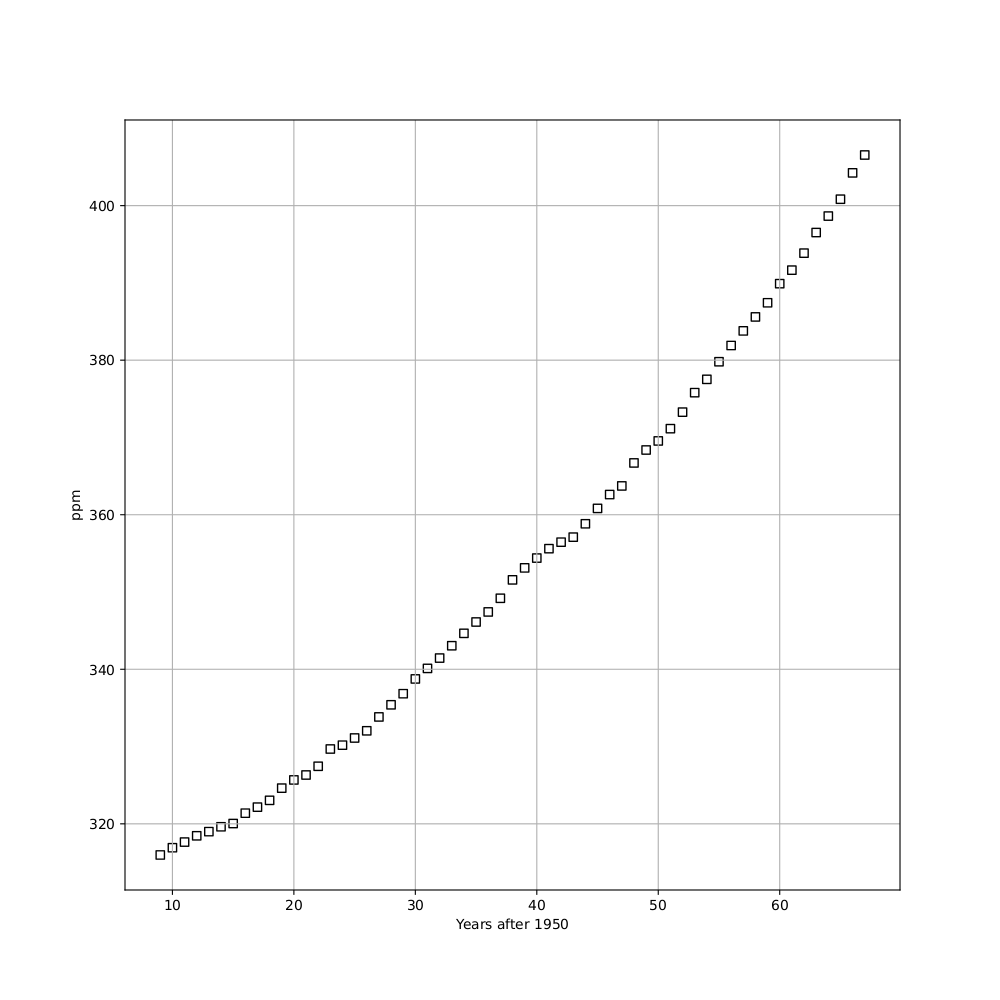
\includegraphics[width=.9\linewidth]{./figures/data.png}
\end{center}

Using the data, we can create a model using NumPy's \texttt{polyfit} function.

\begin{verbatim}
# This code snippet creates the provided model
# as well as generating a new model based on np.polyfit

# Model given in the question for comparison
old_model = np.poly1d([0.01345947, 0.52063260, 310.42336317])
print("Old model:")
print(old_model, "\n")

# Model using newer data
fit = np.polyfit(data["year"], data["mean"], 2)
model = np.poly1d(fit)
print("New model:")
print(model)
\end{verbatim}

\begin{verbatim}
Old model:
         2
0.01346 x + 0.5206 x + 310.4 

New model:
         2
0.01249 x + 0.6027 x + 308.9
\end{verbatim}

With our models ready, we can plot them to compare them visually.

\begin{verbatim}
# This code snippet plots the models
x = np.linspace(min(data["year"]), max(data["year"]), 1000)
scatterplot()
plt.plot(x, old_model(x), color="blue", lw=2)
plt.plot(x, model(x), color="red", lw=2)
plt.savefig("figures/models.png")
\end{verbatim}

\begin{center}
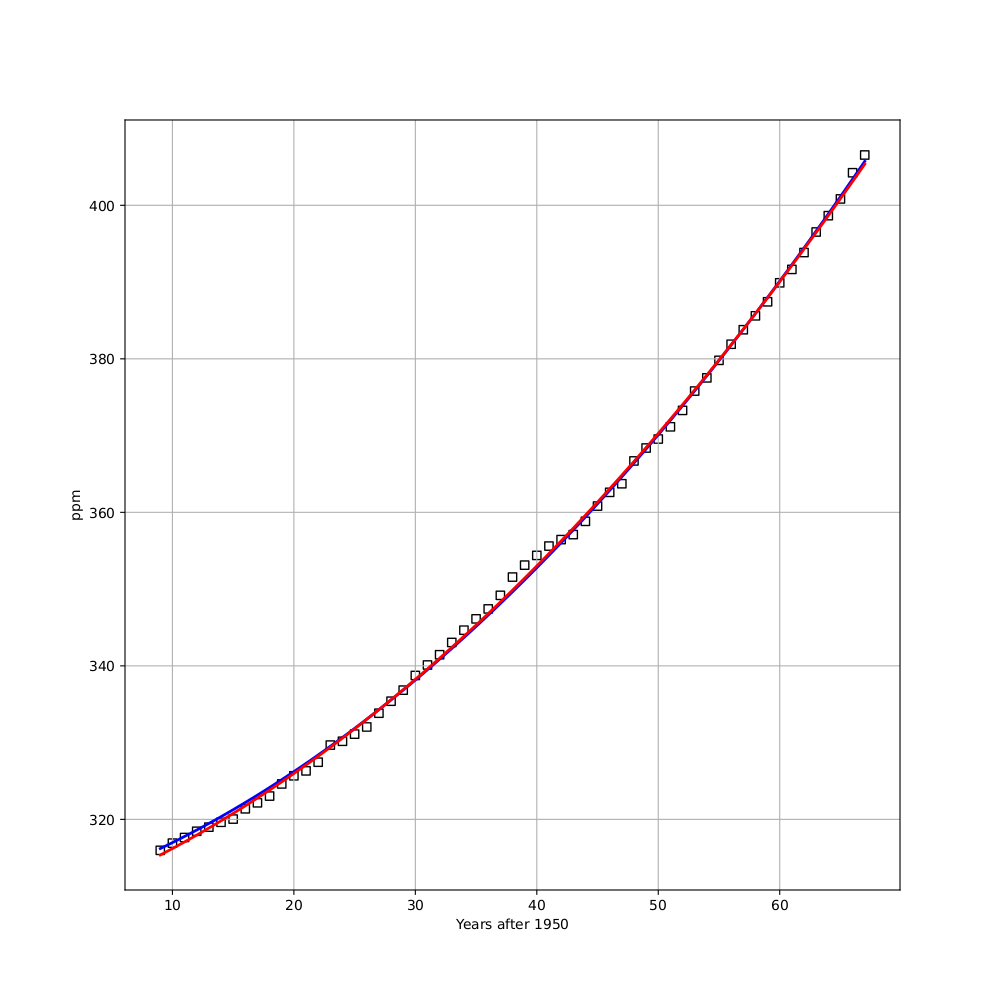
\includegraphics[width=.9\linewidth]{./figures/models.png}
\end{center}

Here, we NumPy provides us with the following model:

\[\hat{y} = 0.01249x^2 + 0.6027x + 308.9.\]

Indeed, this closely matches that of the model provided
to us:

\[\hat{y} = 310.42336317 + 0.52063260x + 0.01345947x^2\]

As an additional check, we can also compare the models
visually using the plots and see that they match each
other when plotted.

\subsection{Question 2}
\label{sec:orgf700d27}

According to the model what will CO\(_{\text{2}}\) levels be in 2050?

\noindent\rule{\textwidth}{0.5pt}

\begin{verbatim}
model(2050 - 1950)
\end{verbatim}

\begin{verbatim}
494.0709782199019
\end{verbatim}

According to the model, there will be approximately
494.071 ppm of CO\(_{\text{2}}\) in the atmosphere by 2050.

\subsection{Question 3}
\label{sec:org0182eb6}

What is the rate of change of CO\(_{\text{2}}\) in 2017
(the last year of the data set) and what is
the percentage rate of change?

\noindent\rule{\textwidth}{0.5pt}

Taking the derivative of the model provided by \hyperref[sec:org98ee15e]{Question 1},
we find the rate of change of CO\(_{\text{2}}\) to be modeled by

\[\hat{y}' = 0.02498x + 0.6027.\]

We can verify this in code:

\begin{verbatim}
rate_of_change = np.poly1d([model.c[0] * 2, model.c[1]])
rate_of_change
\end{verbatim}

\begin{verbatim}
 
0.02497 x + 0.6027
\end{verbatim}

Now all we need to do is use that model to find the
rate of change in 2017:

\begin{verbatim}
q3a = rate_of_change(2017 - 1950)
q3a
\end{verbatim}

\begin{verbatim}
2.276033781313511
\end{verbatim}

So, the rate of change of CO\(_{\text{2}}\) in 2017 is approximately
2.276 ppm/year or 227.6\%.

\subsection{Question 4}
\label{sec:orge7010f3}

Assuming that CO\(_{\text{2}}\) levels continue to grow constantly at the
2017 rates, what will the CO\(_{\text{2}}\) levels reach in 2050?

\noindent\rule{\textwidth}{0.5pt}

If the CO\(_{\text{2}}\) levels were to continue to grow constantly
at the 2017 rates, then we can represent this model
by taking the rate and the CO\(_{\text{2}}\) level at 2017.

\begin{verbatim}
q4_model = np.poly1d([q3a, list(data["mean"])[-1]])
q4_model
\end{verbatim}

\begin{verbatim}
 
2.276 x + 406.6
\end{verbatim}

Plotted, the assumed model would look like this:

\begin{verbatim}
yes
ports both :results none
     x = np.linspace(0, 2050 - 2017 + 5, 100)
     plot_config(xlab = "Years after 2017")
     plt.plot(x, q4_model(x))
     plt.savefig("figures/model-q4.png")
\end{verbatim}

Then the predicted CO\(_{\text{2}}\) level by 2050 would be calculated as so:

\begin{verbatim}
q4_model(2050 - 2017)
\end{verbatim}

\begin{verbatim}
481.6591147833459
\end{verbatim}

So according to this model, the CO\(_{\text{2}}\) level by 2050 will
reach approximately 481.67 ppm.

\subsection{Question 5}
\label{sec:org95871d8}

Atmospheric CO\(_{\text{2}}\) levels of 450 ppm yield a likely chance that
global average temperature increases will be at least \(2^{\circ}\)
Celsius. \footnote{Warren, R. 2006. Impacts of global climate change at different annual mean global temperature increases, in H.J. Schellnhuber et al. (eds.) Avoiding Dangerous Climate Change. Cambridge University Press, Cambridge}
According to the model, in what year do we reach a CO\(_{\text{2}}\) level of 450 ppm?
If we assume CO\(_{\text{2}}\) levels continue to grow constantly at the 2017 rates,
in what year do we reach a CO\(_{\text{2}}\) level of 450 ppm?

\noindent\rule{\textwidth}{0.5pt}

To find the year we reach a CO\(_{\text{2}}\) level of 450 ppm according to the model,
we can translate the model down vertically by 450 and then take the
largest positive root.

\begin{verbatim}
q5a_m1 = np.poly1d([model.c[0], model.c[1], model.c[2] - 450])
q5a_p1 = max(q5a_m1.roots)
q5a_p1
\end{verbatim}

\begin{verbatim}
84.86137790253937
\end{verbatim}

Ensuring that this year indeed corresponds to a CO\(_{\text{2}}\) level of 450 ppm,
we can plug it back into the model.

\begin{verbatim}
model(q5a_p1)
\end{verbatim}

\begin{verbatim}
450.0
\end{verbatim}

We can then repeat the same steps for the 2017 model.

\begin{verbatim}
q5a_m2 = np.poly1d([q4_model.c[0], q4_model.c[1] - 450])
q5a_p2 = max(q5a_m2.roots)
q5a_p2
\end{verbatim}

\begin{verbatim}
19.09022632121249
\end{verbatim}

This produces a very different value.
That is because the 2017 model predicts the CO\(_{\text{2}}\) levels
starting from 2017, however we want a prediction of the
years since 1950, not 2017.
The following calculation will provide us with this.

\begin{verbatim}
2017 - 1950 + q5a_p2
\end{verbatim}

\begin{verbatim}
86.0902263212125
\end{verbatim}

Then we also verify this prediction.

\begin{verbatim}
q4_model(q5a_p2)
\end{verbatim}

\begin{verbatim}
450.0
\end{verbatim}

According to the model, we reach a CO\(_{\text{2}}\) level of 450 ppm
approximately 84.86 years after 1950, so in the year 2034.

If we assume CO\(_{\text{2}}\) levels continue to grow constantly at the
2017 rates, we would reach a CO\(_{\text{2}}\) level of 450 ppm in
approximately 86.09 years after 1950, so the year 2036.

\subsection{Question 6}
\label{sec:org2e4fb62}

Fill in the blank:
In order to avoid reaching 450 ppm of atmospheric CO\(_{\text{2}}\) the
trend in the data would have to become (???Calculus Term???).

\noindent\rule{\textwidth}{0.5pt}

450 as the maximum limit as \(x\) (years after 1950) approaches infinity.

\subsection{Question 7}
\label{sec:orgb99afc8}

Provide a (general or real world related) question that you would
like answered based on your work here.
This should not be something that you could answer yourself with
a little work.

\noindent\rule{\textwidth}{0.5pt}

How could we leverage artificial intelligence to optimize CO\(_{\text{2}}\) emissions?

\subsection{Question 8}
\label{sec:org7100531}

Summarize your work on questions 1-5 in a short paragraph
as if it were a news article

\noindent\rule{\textwidth}{0.5pt}

Carbon dioxide in the Earth's atmosphere is growing at an exponential rate.
This is a concern as atmospheric carbon dioxide has been known to be a
significant factor in climate change on Earth.
Climate change can be devastating, as shown in the description.
My work predicts the amount of atmospheric carbon dioxide for each
year and the rate at which it is produced each year.
Additionally, it visualizes those predictions on graphs generated
by matplotlib.
\end{document}